\subsection{Discussion and Recommendations}
\subsection{Interpretation}
- Nadine
- Comparison fmincon
- KKT conditions checking
- Sensitivities (importance of constraints, variables)


\subsection{Recommendations}
Based on the maximum stress values of both optimizations is safe to assume that the straight interlocking design can outperform the diagonal design.
The maximum stress which can be reached with the straight design is roughly tripple the maximum stress which can be achieved using the diagonal setup.
Even when taking into account inaccuracies in the modeling (as discussed below) the straight design comes out as a clear winner.

The ultimate tensile strength of the interlocking metamaterial microstructure is predicted to be \SI{70}{\percent}
compared to the weaker of the two materials, Ultimaker PolyPropylene.
This value is relatively high compared to the weak chemical bonding between PP and most other thermoplastics.

Given that any manufacturing system has inaccuracies, it might be a good idea to settle on a design which is slightly different from the obtained optimum.
We can assume a deposition accuracy of \SI{0.1}{\milli\meter}, which is a reasonable guesstimate for most desktop FDM 3D printing systems.
The optimum is found at the intersection of several constraint surfaces - each of which has a different steepness at the optimum.
Taking the manufacturing accuracy is a random perturbation in the design space we can envision that the expected stress at the optimum might be lower
compared to a different reference point which is a bit farther down along the least steep surface.
Looking at the graphs and the sensitivities it would make sense to choose a design with a slightly lower $\hf$ and $w^b$ than the optimum of the straight design.
However, a thorough mathematical justification of the exact location of the best point in the design space given manufacturing inaccuracy remains future work.

Depending on the application of the interlocking structure different constraint values might apply.
For different materials the optimum can be quite different.
\todo{Refer to sensitivity wrt $\sigma_a$}
Another important consideration is the design constraint;
for thin designs the value of \SI{3.6}{\milli\meter} might be too big already.
\cref{fig:stress_vs_L} shows that if the design it, using a more lenient design constraint provides dimishing returns.
Moreover, the minimal manufacturable design is already at \SI{84}{\percent} of the ultimate stress compared to twice the total allowed length $\lmax$.

\begin{figure}
	\centering
	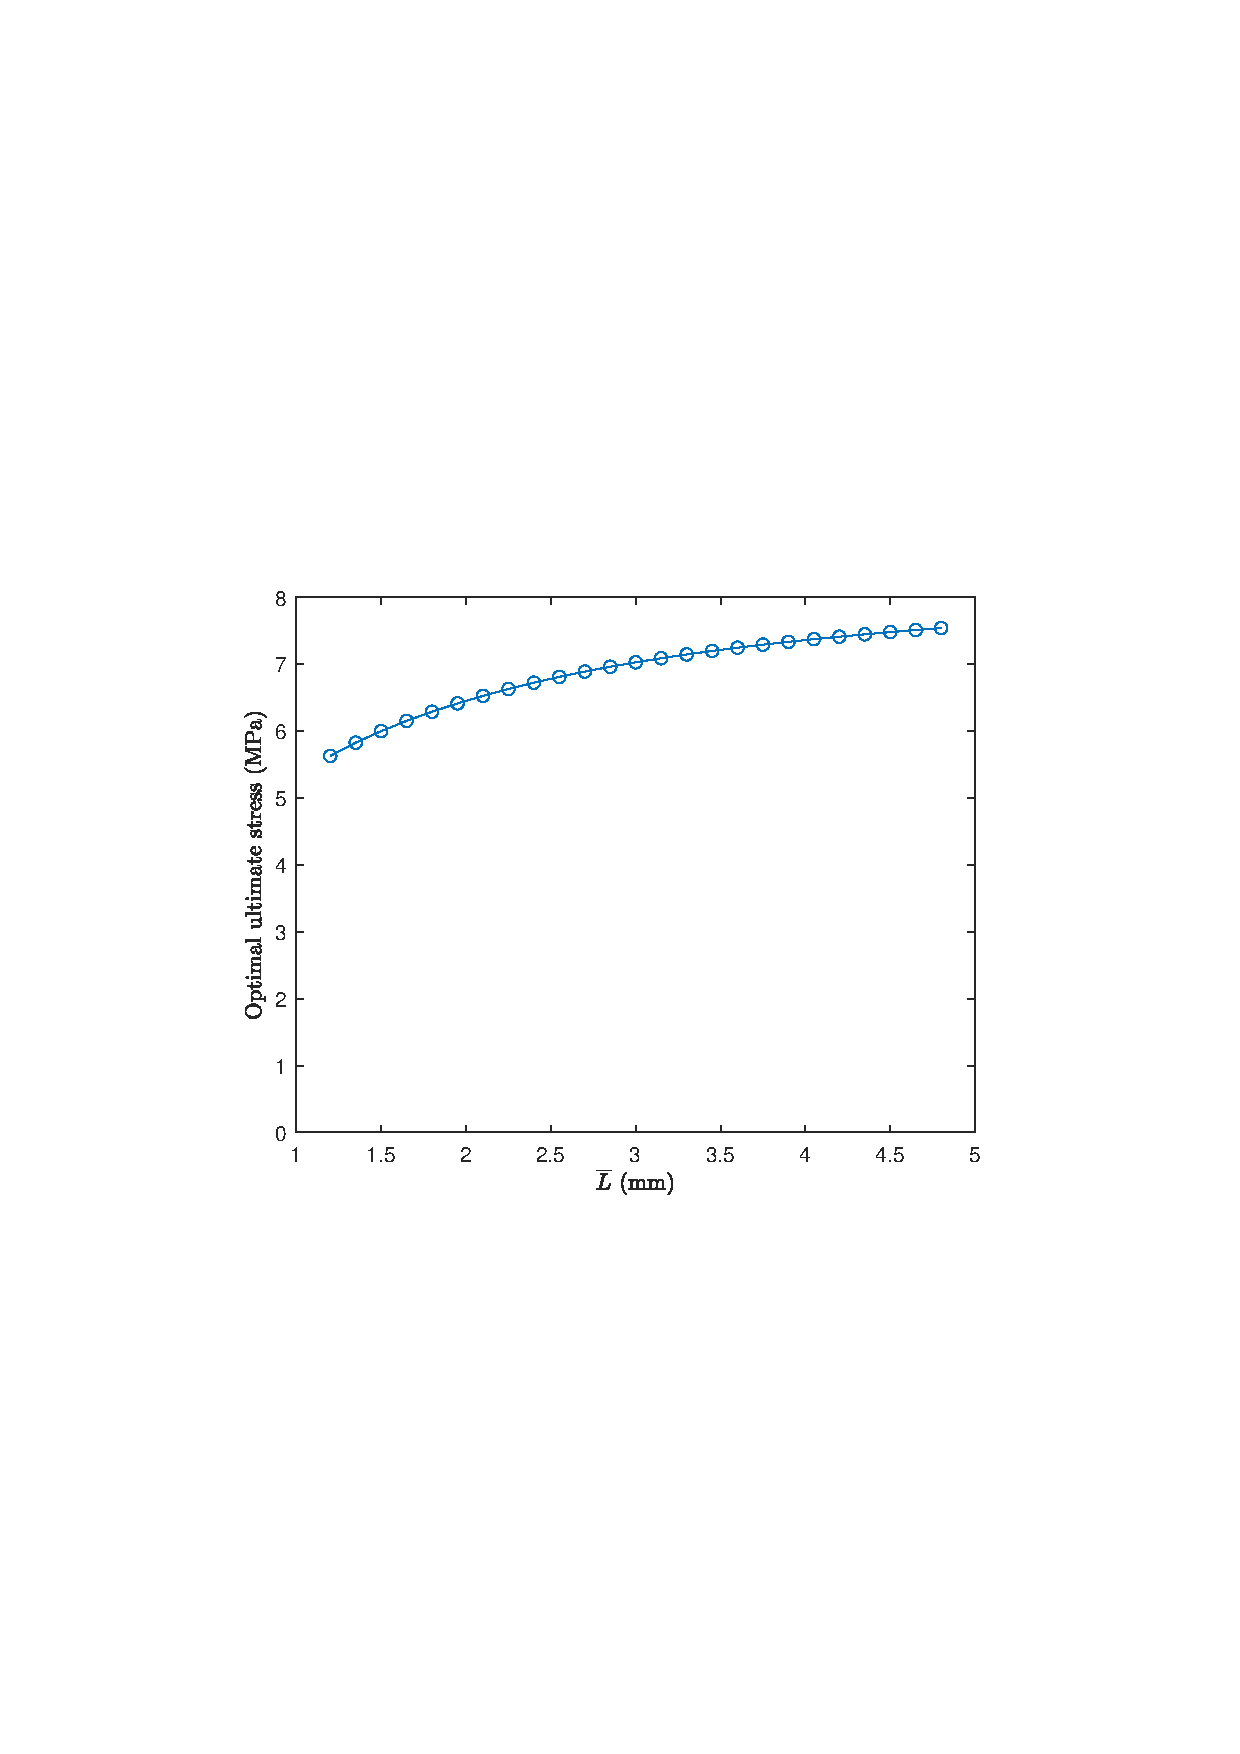
\includegraphics[width=.5\columnwidth]{sources/method/straight_max_stress_different_L.pdf}
	\caption{Optimal stress for various values of the design constraint.}
	\label{fig:stress_vs_L}
\end{figure}


\subsection{Limitations and Future work}
As mentioned before, the active set strategy and the lambda update strategy need more tuning to work properly;
if not with better heuristics then with local iterations to get $\xvec$ and $\lamvec$ closer to their intended values.

The mathematical problem definition we proposed has strong assumptions w.r.t. the homogeneity of stress distributions throughout the part,
while we can expect that in such complex internal loading scenarios the disctribution of stress to be heterogenous.
Specifically the validity of the diagonal model is hard to verify, given that the angles make for a difficult to analyse design.
Also factors such as friction can prove to be significant.

One line of future research is directed at different types of interlocking designs.
Does high genus interlocking designs outperform 2D dovetail type interlocking designs for more flexible materials?
How would the optimal interlocking design look for different forces, like shear, or a vertically applied force?
